\documentclass[12pt]{article}
\usepackage[margin=1in]{geometry}
\usepackage{enumitem}
\usepackage{titlesec}
\usepackage{parskip}
\usepackage{graphicx}
\usepackage{hyperref}
\usepackage{fontenc}

\title{\textbf{Powell 2000 RG Notes}\\
\large Powell, G. Bingham Jr. \textit{Elections as Instruments of Democracy: Majoritarian and Proportional Visions}.\\
New Haven: Yale University Press, 2000.}
\author{}
\date{}

\begin{document}

\maketitle

\section{Main Idea}

There are two primary frameworks (and institutional structures) through which elections can define democratic governance: majoritarian, and proportionalistic. In a majoritarian approach, the government is bound to directly reflect the interest of the party receiving a majority of seats (though this may not always imply a majority of votes), and provides a rather ``all-or-nothing'' approach to representation. Conversely, in a proportionalistic system, the government ideally reflects the proportionate makeup of policy preferences and perspectives throughout the voting population, and delivers policy influence in line with those proportions. Oftentimes, the proportional approach provides better voter-representative congruency and fairer policy representation as compared to the majoritarian lens. It further tends to more effectively protect minority interests, and in particular can help balance policymaking. Yet, majoritarian governance implicitly improves voter-policy congruence. That is, while proportionalism can deliver a legislature that most effectively reflects the people, it may not empower such legislatures to be meaningfully effective in any broadly-improving way.



%--------------------------------------------------
\section{General Notes}
%--------------------------------------------------

\begin{itemize}[leftmargin=*, itemsep=4pt]
    \item Primary distinction between democratic approaches: \emph{control} over policymakers or \emph{influence} over policy. Each corresponds to a certain ``grand vision'' of electoral accountability:
    \begin{itemize}
        \item \underline{Majoritarian}: The majority should have a near-absolute right to rule, and policy should proceed in accordance with the majority's wishes. Focuses on a relationship of power between voters and their elected officials, whereby voters become ``principals'' who seek to either reward or control their representatives. Consistent with the ``control'' narrative. Centralization of power follows from this, and the primary role of the citizen is to enforce consequences during elections.
        \item \underline{Proportionalism}: The will of each group should be reflected in policy in accordance with the relative size of that group. Focuses on a relationship of influence whereby policy is swayed in a degree proportionate to the relative power of that group, subsequently protecting minority welfare at the expense of direct control over the political system. Consistent with the ``influence'' narrative. Considers elections to be clumsy/noisy signals, and prioritizes universal input without giving an oversized benefit to the majority group
    \end{itemize}
    \item Voters' roles can be roughly perceived as either retrospective or prospective. If retrospective, more aligned with majoritarianism: the voter either punishes or rewards incumbents with their vote (or lack thereof), based on the observed quality of their tenure. If prospective, more aligned with proportionalism: the voter seeks credible commitments from candidates and has some expectation of their performance.
    \begin{center}
        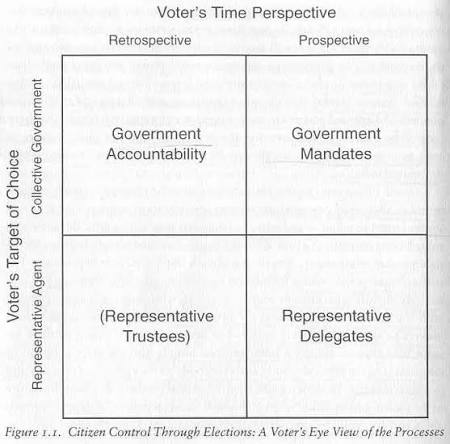
\includegraphics[width=10cm]{powell fig 1.1.jpeg}
    \end{center}
    \item The result of this broader differentiation is two metrics of electoral success: (1) responsiveness to elections in choosing policymakers, and (2) representational congruence between the policymakers' positions and the citizens' preferences. Majoritarianism \emph{should} do better with (1), and proportionalism better with (2).
    \item Election rules in SMDP systems generally limit the number of seats and subsequent equilibria features limited numbers of viable candidates based off of those seats (see Duverger). This can create a significant disproportion in representation amongst majoritarian systems: a 49\% share may ultimately be entirely unrepresented in a legislature. High effective thresholds -- explicit or systemic vote share requirements in order for a party to gain representation -- benefit a majoritarian perspective. As the effective threshold increases, the expected vote-seat disproportionality increases as well.
    \item ``If the decision rules encourage or require the government parties to negotiate with independent groups in the assembly, especially those representing voters who supported different parties, I want to characterize them as closer to the proportional vision. If the decision rules encourage the government parties to control the executive and the assembly without check or division, I characterize them as majoritarian.''
    \item ``Influence of the opposition'' from Strom -- largely based on the role and importance of committees. Presence is important, of course, but further considerations: do the committees have policymaking power? Is there any veto opportunity for minority parties within committees? Are the committees highly specialized such that mainstream ideological backgrounds of certain parties can be effectively cast aside? Committees as a primary metric of decentralization
    \item Though constitutional design and legislative rules can change over time, their change in democracies is usually not particularly drastic or quick, for a number of reasons including institutional safeguards. But, an additional -- and potentially strongest -- consideration: an incumbent usually has won office through some means of benefitting from the system in place, and therefore has minimal incentive to change it. This is a more self-serving equilibrium outcome than a Dahl ``trust in the opposition'' framework, and rather suggests tautologically that the system usually has worked for whoever is currently in power.
    \item A core component of restrospective voting requires that the citizens are able to perceive who should be held accountable for what decisions. Though this may be obvious in some more direct settings -- and majoritarian systems provide a great deal of transparency -- it becomes a bigger issue with coalition governments. Powell finds that the extent to which voters treat an in-government party as responsible for policy throughout their incumbency is contingent on their position within the coalition as well as whether or not they ruled individually or with other parties.
    \item Party mandates stem from a majoritarian perspective whereby the government's winning of a majority of votes/seats/etc. provides it with both the ability and the responsibility to fully deliver on its visions, even occasionally with disregard for institutional safeguards or compromises. Mandates ``assume a single decisive choice'' and generally simplify policy into one dimension; this is potentially an over-simplification that blurs their ability to govern appropriately on less-salient concerns.
    \item Control through mandates requires two stages:
    \begin{enumerate}
        \item ``The voter needs to be able to identify the prospective future governors and have some idea of what they will do if elected. This condition is necessary if the voters are to make good prospective choices.'' Calls them ``\emph{identifiable prospective governments}"
        \item ``The outcome of the election should bring into office a coherent government committed to policies that correspond to the voters' anticipations and capable of carrying them out. Calls them ``\emph{a responsively formed working majority after the election}''
    \end{enumerate}
    \item ``In the nineteenth-century context having a voice in the legislature may have seemed sufficient. But the emergence of extremely cohesive legislative parties and the dominance of many parliaments by their executives imply to those concerned about them the desirability of giving minorities some greater weight in policy making than merely the opportunity to be heard in (largely irrelevant) legislative debate.'' That is, PR protects minority interests to a better extent than majoritarianism. Yet, simple resolutions to this often come at a great normative cost: empowering minorities to enact vetos is likely inherently undemocratic, and any pathway leaves plenty of opportunities to be abused.
    \begin{itemize}
        \item ``Given that citizens' preferences are appropriately articulated by the parties they choose to support in the election, there remain two conditions: that each party win fair representation in the assembly and that it have fair influence in policy making."
    \end{itemize}
    \item Finds general support for PR particularly wrt effective authorized representation: tends to provide unilaterally-improved representation compared to MAJ systems. The work of course considers this conclusion to be nuanced, but an important consideration in constitutional design.
    \item Responsiveness is not the only metric of successful democracy and in fact may often be in conflict with other measures of success. Consider abuse of majoritarianism, lack of delegation to public policy experts, etc. Two hypotheses for responsiveness:
    \begin{enumerate}
        \item ``The majoritarian vision relies on elections featuring few competitors and identifiable future governments during the election and majority governments that thoroughly control policy making after the election.... A single party wins a majority of votes, controls the legislature, and makes policy. Governments can claim voter mandates for their election promises and are clearly responsible for their actions.''
        \item ``The proportional vision implies its own hypotheses about responsiveness. This vision stresses the superiority of all citizens and the need for rules that fairly reflect the choices of citizens in the composition of the legislature. The legislature suffers from neither overweighting of some parties at the expense of others nor forced cohabitation within individual parties or preelection coalitions that can freeze bargaining opportunities.''
        
        \begin{center}
        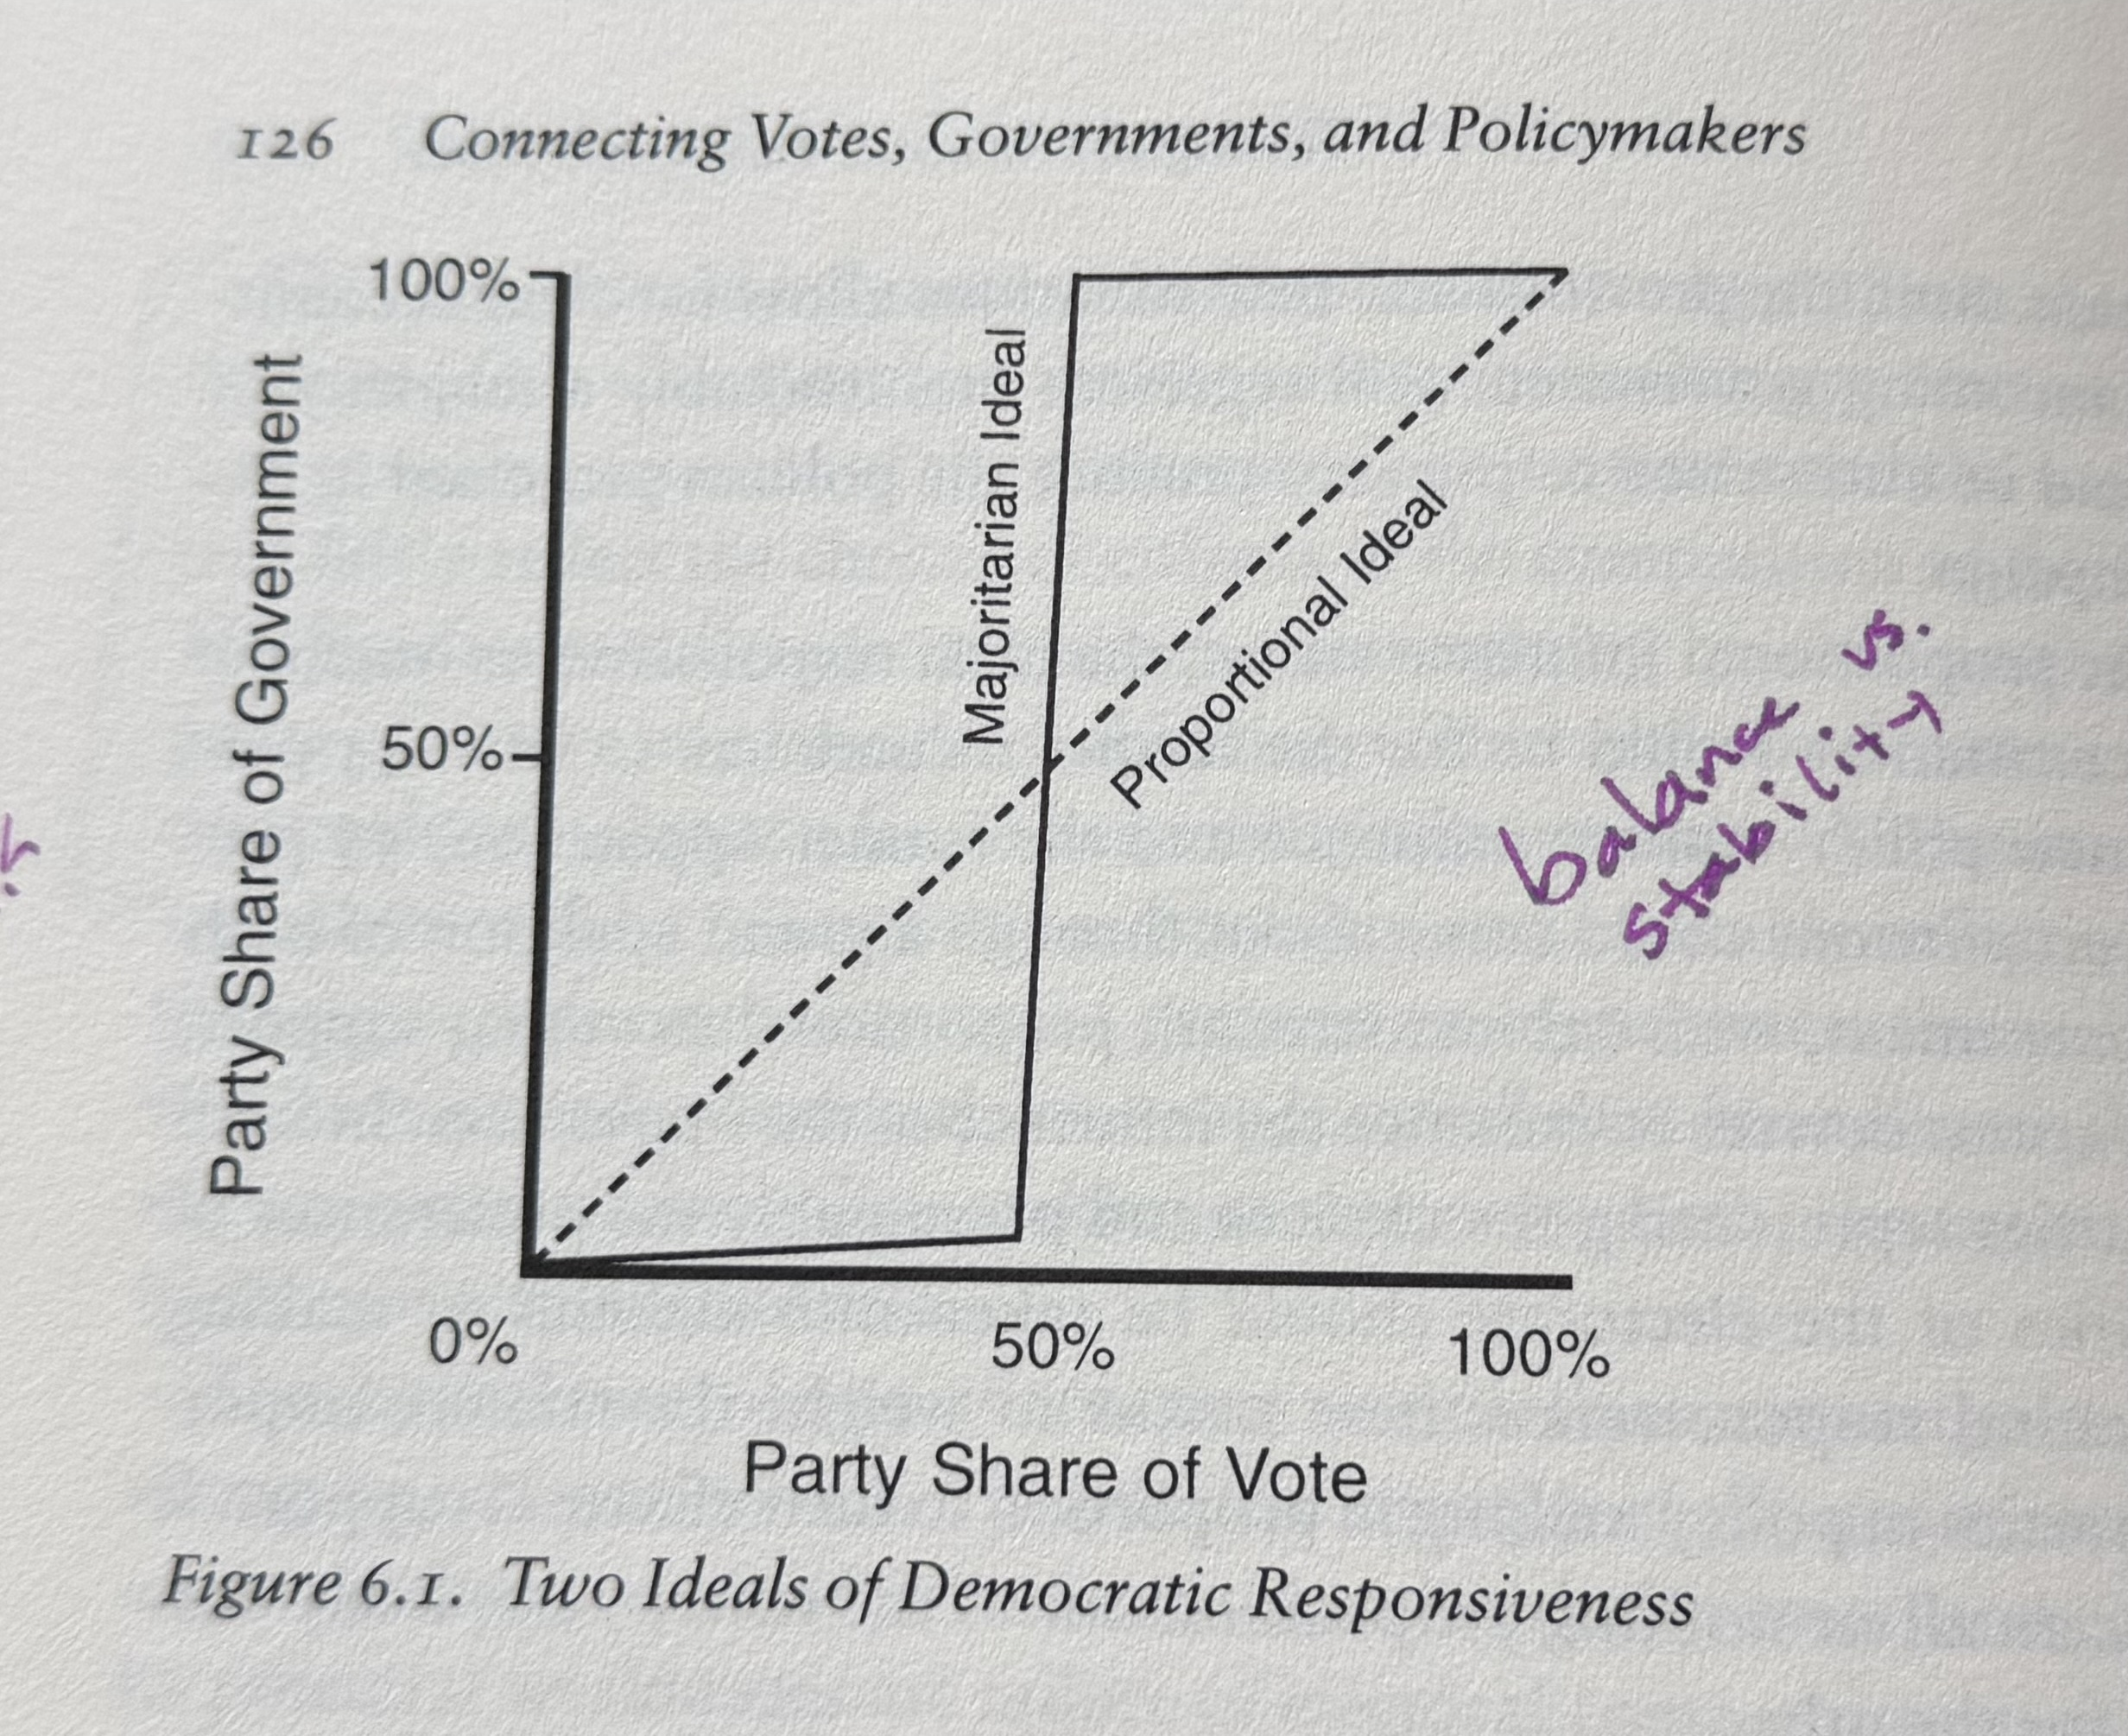
\includegraphics[width=10cm]{Powell Fig 6.1.jpg}
        \end{center}
    \end{enumerate}
    \item Party vote and policy-making share are generally much more aligned under a PR system than majoritarian (see below section for more details on distortion). 
    \item The decisive stage of citizen preferences in the majoritarian model is the election itself -- yet, in the proportionalistic view, it is multistage. Citizens are represented once in the individual election, and then again in coalition bargaining between parties if no outright majority is achieved.
    \item A proportionality approach \emph{can} improve voter-policy congruence; a majoritarian approach \emph{does} improve it. ``In situations in which a single party or coalition of parties forms a government and must maintain tight party discipline, which empirically is the case in almost all parliamentary systems, the govern,ment might be expected to make policies that correspond not to the legislative median but to its own internal distribution.''
    \item ``Why do majoritarian processes so often fail? One answer is that despite the apparenet robustness of the theoretical connections, correspondence depends in fact on achieving some very specific conditions and, importantly, that it is the nature of the majoritarian processes that fairly small deviations from these lead to large, undesirable consequences. A second answer is that it frequently is asking too much of elections that in a complex world they bear the full, decisive burden of connecting voters and policymakers as the majoritarian vision presumes.''
\end{itemize}


\section{Important Specific Factual Claims}

\begin{itemize}[leftmargin=*, itemsep=4pt]
    \item Making retrospective judgments requires some clarity about specifically \emph{who} made \emph{what} judgments. Requires both some degree of transparency and a sense of consistency from amongst the citizens, who in turn need to accurately perceive the dynamic at hand. This adds an additional dynamic to be considered: \underline{clarity of responsibility}
    \item Focuses on two alternative methods of connection between citizen preferences and the formation of policy coalitions (and subsequently policy): differentiating factor is whether or not a voter's vote is sufficient to fully express their preferences. This may not be the case precisely because voters are presented with an exclusive menu, rather than empowered to fully express their specific preferences over a continuous domain.
    \item Possible veto institutions to restrict a national assembly's power:
    \begin{enumerate}
        \item Independent executives (main example is USA)
        \item Separate legislative chamber with independenet selection base and veto powers
        \item Federal systems: regional checks on centralized power
        \item Judicial review (think Vanberg) -- court system (usually independent) has some oversight over legislative process
    \end{enumerate}
    \item Majoritarianism provides a degree of quantitative stability in election result shifts: a tiny change in vote margin is unlikely to result in a regime change in a majoritarian system, while a proportionalist system may be much more volatile to such changes
    \item Party mandates ``seems to have appeared at the end of the nineteenth century as the first mass political parties, usually Socialist parties, were mobilizing new electorates in Western Europe.... They argued, moreover, that, having made policy commitments to the electorate, they were both authorized and obligated to carry out those policies once in office. This formulation translated the older concept of majoritarian or populist democracy into terms that took explicit advantage of the enfranchisement of mass electorates and the emergency of mass political parties."
    \item Majoritarian systems are more likely to allow for severe distortion whereby a majority of votes does not result in a majority of seats (by clumping votes within districts, etc.) because of its all-or-nothing nature. However, this sort of distortion -- though possible -- is much less common within PR systems, as there are fewer opportunities for broad deviations. Unlikely to see minority-vote-holders become majority-seat-holders in a proportional system (that is, outright -- does not consider inclusion in a coalition government, which is its own consideration).
    \item Two types of responsiveness failures:
    \begin{enumerate}
        \item ``Those in which failing to meet one ideal draws the election outcome closer to the alternative ideal''
        \item ``Unmitigated failures, in which distance from one ideal does not draw the outcome toward the alternative''
    \end{enumerate}
\end{itemize}


\section{Connections}

\begin{itemize}
    \item Figure 1.2 (pg. 15) should link directly to Dahl: begin with citizen preferences/beliefs, flow to policy
    \item Many references to (and in agreement with) Lijphart 1984, who differentiates two approaches to democratic government: either the government should be responsive to the majority (Westminster approach), or should be responsive to ``as many people as possible."
    \item ``The effective representation of voters for opposition parties is always less than that of voters for governing parties, but the degree of difference varies, depending on the bargaining resources of those parties.'' $\rightarrow$ very reminiscent of Dahl's polyarchy argument: is the opposition competitive, and is the political system competitive as a whole?
    \item Connection to Carey (2009) and Larreguy \& Raffler (2025) regarding different models of accountability, etc. Likely a tie between majoritarianism and the rise of social media being against it, but the pros of majoritarianism are therefore degraded
    \item Boix 1999: mainstream parties use the transition from majoritarianism to PR as a means of protectionism when a new party (often socialist) emerges -- but, this requires the ability to consolidate around a given establishment party, which can be difficult / impossible if the ruling parties are relatively comparable in size and influence
    \item Diermeier \& Vlaicu 2011: discuss majoritarianism as a reflection of pivotal politics, and further expand on how it can be sustained even in the absence of formal party organizations
    \item Gandhi \& Przeworski 2007: further expansion of the "mandated right to rule" within authoritarian systems, whereby autocrats allow for some dissent (particularly by means of inclusive legislatures) such that their power can actually be further consolidated due to the additional credible threats they have lent
\end{itemize}


\section{My Critiques}

\begin{itemize}
    \item Doesn't seem to particularly explore the geographic aspect here: proportionality makes it much harder to have individual district representatives who are accountable for certain aspects, etc, without making the number of delegates huge (or the number of districts small). It seems possible that a PR approach may simply not be effective in smaller political bodies where granularity cannot be achieved while holding direct accountability.
    \item Discusses the inherent stability of majorities, given that few fall apart post-election -- but, isn't this somewhat tautological? Aren't these systems unlikely to collapse simply because there is virtually no institutional means by which this can happen? Perhaps this also follows from a Duverger's application, but in a two-party legislature, it is presumably rare (though not impossible) that a schism in one party results in absorption by the other...
\end{itemize}


\end{document}
